\documentclass[12pt]{report}

%Vous souciez pas de tout les packages, j'ai oublié ce que fait la moitié d'entre eux

\usepackage[utf8]{inputenc}
\usepackage[T1]{fontenc}
\usepackage[francais]{babel}
%\usepackage{layout}
\usepackage[left=3cm,right=3cm,top=3cm,bottom=3cm]{geometry}
%\usepackage{setspace}
\usepackage{soul}
\usepackage[normalem]{ulem}
%\usepackage{eurosym}
%\usepackage{bookman}
%\usepackage{charter}
%\usepackage{newcent}
%\usepackage{lmodern}
%\usepackage{mathpazo}
%\usepackage{mathptmx}
%\usepackage{url}
%\usepackage{verbatim}
%\usepackage{moreverb}
%\usepackage{listings}
%\usepackage{fancyhdr}
%\usepackage{wrapfig}
\usepackage{color}
%\usepackage{colortbl}
\usepackage{amsmath}
\usepackage{amssymb}
\usepackage{mathrsfs}
%\usepackage{asmthm}
%\usepackage{makeidx}
\usepackage{graphicx}
\usepackage{tabularx}
\usepackage{tgtermes}
\usepackage{titlesec}
\usepackage[final]{pdfpages} 
\usepackage{epsfig}
\usepackage{comment}
\usepackage{float}
\usepackage{amsmath}
\renewcommand{\emph}{\textit}
\renewcommand{\thesection}{\arabic{section}}
\renewcommand{\thesubsection}{\arabic{section}.\arabic{subsection}}
\titleformat*{\subsection}{\bfseries}
\parskip=5pt

%Information pour la page de garde

\title{TP3 et 4 - Estimation d'une homographie}
\author{Jean-Baptiste \bsc{Morice}, Guillaume \bsc{Versal}}
\date{\today}

\begin{document}

%Commande qui crée la page de garde
\maketitle

%\tableofcontents

\newpage
\section{Introduction}

L'objectif de ces deux TP était de manipuler le concept d'homographie en vision par ordinateur. Dans ce contexte une homographie est une fonction permettant de projeter les points correspondants d'un premier plan image vers un second dans un système de stéréovision. 

\section{Notre travail}

\subsection{Question 1}

On cherche ici à appliquer l'algorithme Direct Linear Transform pour estimer une homographie. Pour savoir combien de points, au minimum, sont nécéssaires pour la calculer il faut se réporter à l'équation que l'on cherche à résoudre :

\begin{center}
$x_2 = H^2_1x_1 $ qui est équivalente au produit vectoriel $x_2$ x $H^2_1x_1 = 0$
\end{center}


Où $x_1$ et $x_2$ représentent les coordonnées de deux points respectivements dans les plans images 1 et 2. Et $H^2_1$ la matrice d'homographie entre les plans image 2 et 1.

On peut reformuler cette équation sous la forme du système suivant :

\begin{center}
$
\begin{pmatrix}
 & ... & \\ 
0^T & -w_{i2}X_1^{iT} & y_{i2}X_1^{iT}\\ 
w_{i2}X_1^{iT} & 0^T & -x_{i2}X_1^{iT}\\
 & ... & 
\end{pmatrix}
\begin{pmatrix}
h_1\\ 
h2\\ 
h3
\end{pmatrix}
= 0
$
\end{center}

Avec le point $x_2=(x_2, y_2, w_2)$ en coordonnées homogènes, ainsi que $X_1^T$ le vecteur colonne des coordonnées homogènes du point $x_1$ transposé. Et $h_1$, $h_2$ et $h_3$ des vecteurs colonnes de taille 3 correspondant aux lignes de la matrice $H^2_1$.
La paire de lignes de la matrice de gauche est répétée pour chaque point dont on connait la correspondance entre les deux images. On résondra ensuite ce système par une décomposition en vecteurs propres.

Ainsi, on voit donc bien qu'il nous faut un minimum de 5 points pour obtenir une solution.

\subsection{Question 2}

Pour construire une fonction permettant d'estimer l'homographie nous avons donc implémenté la résolution du système décrit dans la réponse à la question précédente.

\subsection{Questions 3 et 4}

Comme on sait que la matrice d'homographie est inversible, et comme une matrice dont le déterminant est nulle n'est pas inversible, une mesure de qualité possible serait de calculer ce dernier. La proximité du déterminant avec 0 nous donnerait ainsi une idée de la qualité de l'estimation.

On pourrait également vérifier la conservation de l'échelle et des transformations entre les plans.

Néanmoins, façon la plus triviale pour juger de la qualité serait d'appliquer ce qui est proposé à la question 4. C'est à dire de calculer la distance entre la projection d'un point donnée par la matrice d'homographie estimée et la position connue visuellement de ce point.

Cette méthode appliquée aux résultats produits par notre algorithme de DLT nous donne les résultats suivant :

\begin{figure}
\begin{center}
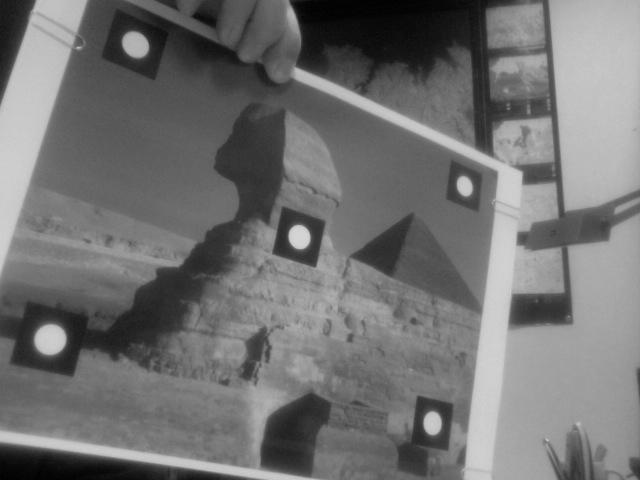
\includegraphics[scale=0.3]{Images/I1.jpg}
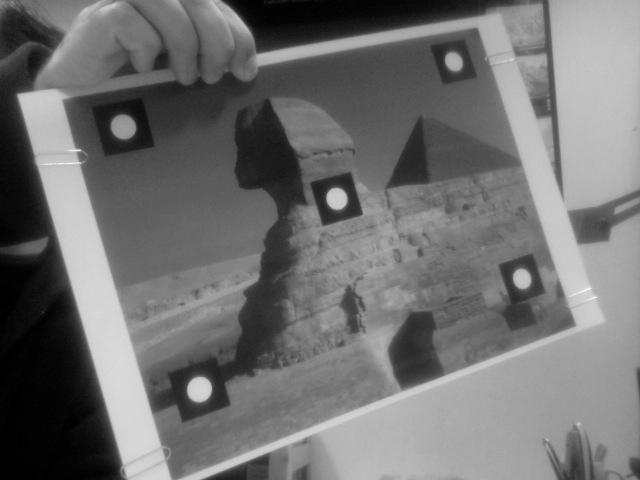
\includegraphics[scale=0.3]{Images/I2.jpg}
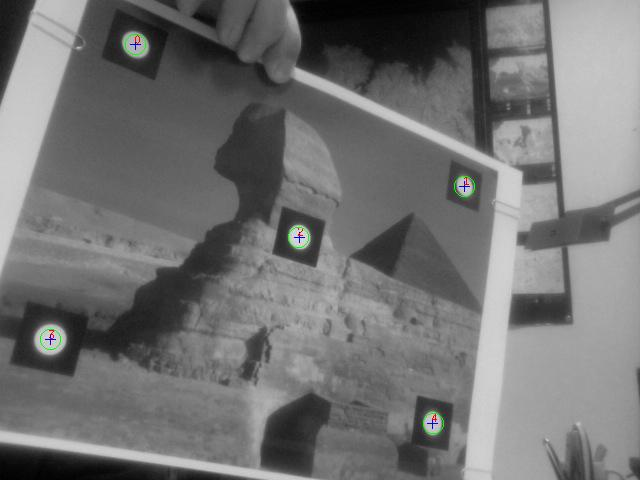
\includegraphics[scale=0.3]{Images/result_tp3.jpg}
\caption{Erreur distance entre l'estimation et la réalité}
\end{center}
\end{figure}

Les images du haut sont celles utilisées pour simuler notre système de stéréovision. Sur chacune d'elle on a selectionné manuellement cinq points au centre des pastilles blanches. Ces points sont supposés être le projetés l'un de l'autre dans les deux images, si l'on néglige l'erreur humaine lors de la sélection. Ce sont ces points que l'on a utilisé pour estimer l'homographie. Les rayons des cercles verts sur l'image du bas représentent la distance, multipliée par dix pour que cela soit plus visible, entre la position donnée par notre matrice d'homographie estimée et la position captée à la souris.

\subsection{Question 5}

Nous avons ensuite utilisé la matrice d'homographie estimée pour projeter tous les points de l'image de droite vers l'image de gauche.

\begin{figure}
\begin{center}
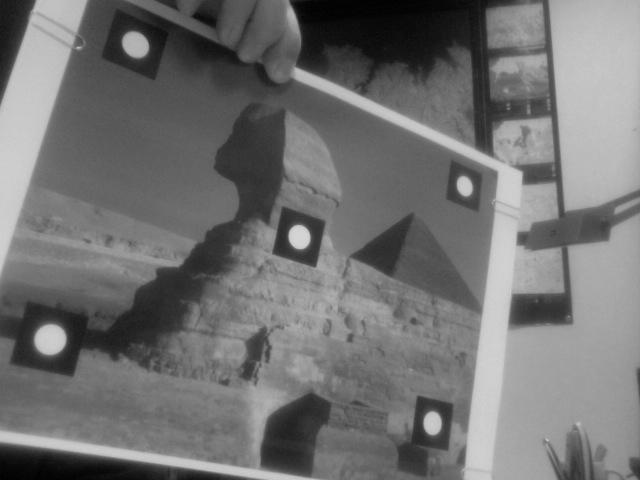
\includegraphics[scale=0.3]{Images/I1.jpg}
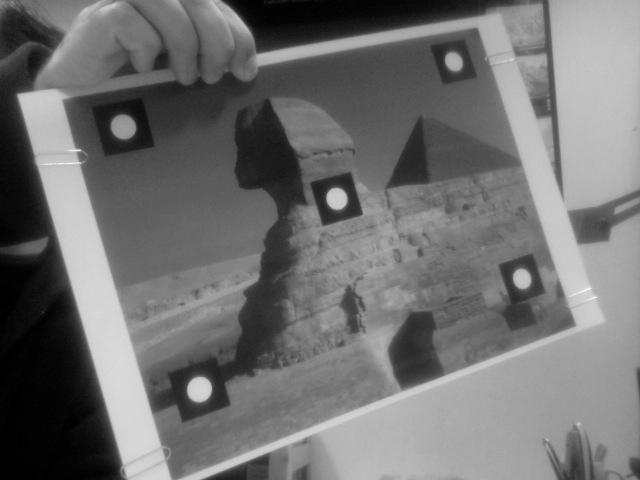
\includegraphics[scale=0.3]{Images/I2.jpg}
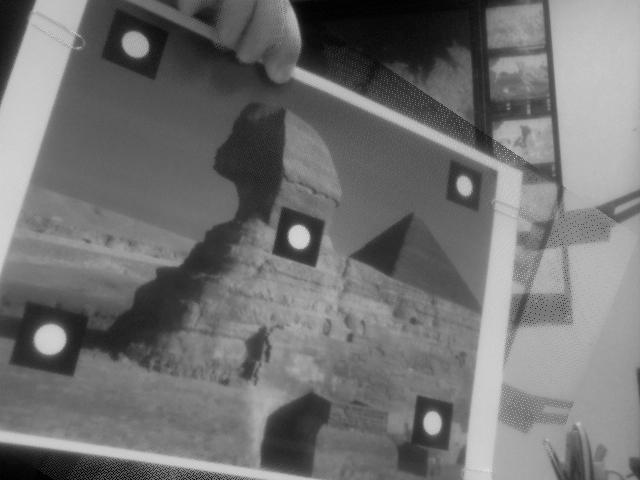
\includegraphics[scale=0.3]{Images/transfer_result_tp3.jpg}
\caption{Transfert des points de l'image de droite vers celle de gauche}
\end{center}
\end{figure}

On observe un artefact autour de l'image du sphinx tenue par la personne, qui correspond au poster accroché sur le mur en arrière plan. Cet effet s'explique par le fait que l'homographie suppose que l'on examine un plan à l'infini, or notre sélection de points a été faite sur le plan de l'image du sphynx, et non pas sur l'arrière plan.


\subsection{Question 6}

Une liste de points d'intérêt correspondants extraits grâce à un SIFT nous sont fournies.

\begin{figure}
\begin{center}
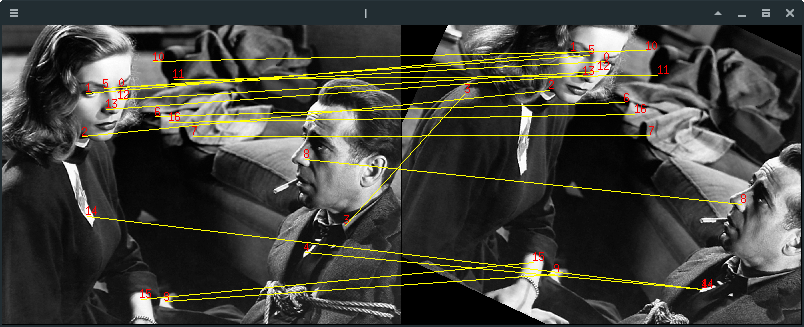
\includegraphics[scale=0.6]{Images/correspondance.jpg}
\caption{Correspondance entre les points détéctés}
\end{center}
\end{figure}

En observant la mise en correspondance des points on constate que deux paires de points sont fausées, celles numérotées 3 et 14. La première va du col de l'homme à celui de la femme et la deuxième va du chemisier de la femme à la chemise de l'homme.

\subsection{Question 7}

Si l'on applique la DLT sur cet ensemble de point et qu'on observe l'erreur de la manière décrite précedemment, on obtient le résultat suivant :

\begin{figure}[H]
\begin{center}
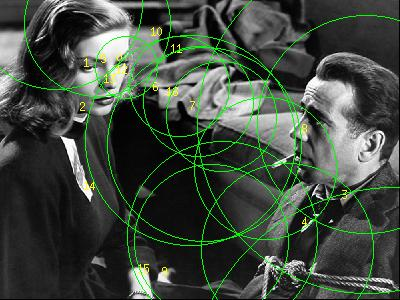
\includegraphics[scale=0.6]{Images/result_dlt_tp4.jpg}
\caption{Erreur distance entre l'estimation et la réalité pour tous les points détéctés}
\end{center}
\end{figure}

On constate donc que les deux paires de points que nous avions identifiées comme fausées ont une grande influence sur la qualité de notre estimation de l'homographie et rendent le résultat inacceptable.

\begin{figure}[H]
\begin{center}
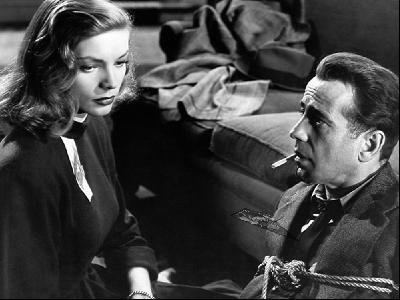
\includegraphics[scale=0.6]{Images/transfer_result_dlt_tp4.jpg}
\caption{Transfert avec l'estimation pour tous les points détéctés}
\end{center}
\end{figure}

Si l'on observe le résultat du transfert des points avec cette estimation de l'homographie on remarque un artefact au centre du torse de l'homme.

\subsection{Question 8}

Pour contourner ce problème nous avons implémenté l'algorithme RANSAC qui permet d'éliminer les données abhérantes de notre ensemble de points. En l'éxecutant sur le même jeu de données nous obtenons le résultat suivant :

\begin{figure}[H]
\begin{center}
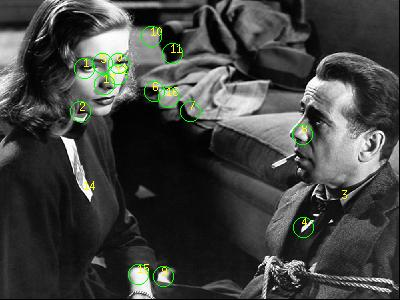
\includegraphics[scale=0.6]{Images/result_ransac_tp4.jpg}
\caption{Erreur distance entre l'estimation et la réalité pour tous les points donnés par RANSAC}
\end{center}
\end{figure}

On constate donc que les deux paires de points que nous avions identifiées comme fausées ont été exclues de l'estimation de l'homographie et que, par conséquence, notre résultat est de bien meilleure qualité.

\begin{figure}[H]
\begin{center}
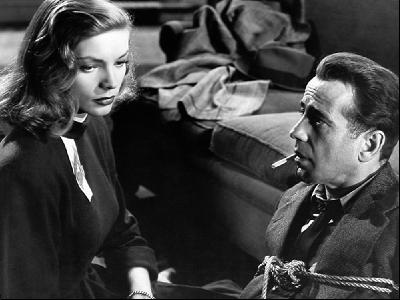
\includegraphics[scale=0.6]{Images/transfer_result_ransac_tp4.jpg}
\caption{Transfert avec l'estimation pour tous les points détéctés}
\end{center}
\end{figure}

Si l'on observe le résultat du transfert des points avec cette estimation de l'homographie on constate que l'artefact du résultat précédent n'est plus présent.

\subsection{Question 9}

Nous ne disposons de ressources nécessaires pour réaliser cette mosaïque mais si on les avait il suffirait pour une séquence d'image donnée de prendre les deux premières, d'extraire des points d'intérêt grâce à un détecteur comme SIFT, d'estimer leur homographie, puis de les fusionner, et répéter le processus avec l'image obtenue et l'image suivante dans la séquence jusqu'à la fin.

\section{Conclusion}
 
Ce TP nous a permis de nous familiariser avec le concept d'homographie, et plus généralement comment l'estimer et évaluer sa qualité dans un système de stéréovision. Les transferts de points que nous avons éffectués posent également les bases des techniques de mosaicking. 

\begin{comment}

%Commande pour le sommaire

\renewcommand{\contentsname}{\large Sommaire} % Change le nom en sommaire
\setcounter{tocdepth}{2} % Défini la profondeur d'une table des matières
\tableofcontents
\newpage

\end{comment}

\newpage


%Commande pour le sommaire des figures

\renewcommand*\listfigurename{\large Liste des figures}
\listoffigures
\newpage


\end{document}
